\section{Implementacion del Sistema BezierComparador}
\label{sec:implementacion}

En esta seccion se describe la implementacion completa del sistema \textit{BezierComparador}, abarcando las tecnologias seleccionadas, la arquitectura de software basada en el patron Modelo--Vista--Controlador (MVC), el diagrama de clases, las convenciones de nomenclatura, el manual de usuario de la interfaz grafica y las decisiones de diseno de la experiencia de usuario (UI/UX).

\subsection{Tecnologias Utilizadas}
\label{subsec:impl_tecnologias}

El desarrollo del sistema se realizo empleando el siguiente conjunto de tecnologias, seleccionadas por su compatibilidad con los requerimientos de rendimiento, precision y construccion de interfaces graficas de escritorio:

\begin{table}[H]
\centering
\caption{Tecnologias y herramientas empleadas en el desarrollo de BezierComparador.}
\label{tab:impl_tecnologias}
\begin{tabular}{p{3.8cm} p{10.5cm}}
\toprule
\textbf{Tecnologia} & \textbf{Justificacion de Uso} \\
\midrule
Lenguaje C\# & Lenguaje orientado a objetos con tipado fuerte y soporte nativo para aritmetica de punto flotante en \texttt{double} (64 bits) y \texttt{decimal} (128 bits), lo cual resulta esencial para las pruebas de estabilidad numerica. \\
\midrule
Windows Forms & Framework de interfaz grafica que proporciona acceso directo al objeto \texttt{Graphics} de GDI+ para el dibujo personalizado con \texttt{DrawLine}, \texttt{FillEllipse} y \texttt{DrawString}, sin depender de funciones predefinidas de curvas. \\
\midrule
.NET 8.0 / 10.0 & Plataforma de ejecucion con deteccion automatica del SDK instalado (\texttt{net8.0-windows} a \texttt{net10.0-windows}), compilacion JIT optimizada y soporte para \texttt{async/await} en la ejecucion de experimentos sin bloquear la interfaz grafica. \\
\midrule
\texttt{System.Diagnostics.Stopwatch} & Temporizador de alta resolucion basado en el contador de rendimiento del hardware del procesador (QPC), con precision de microsegundos, utilizado para medir exclusivamente el tiempo del calculo matematico. \\
\bottomrule
\end{tabular}
\end{table}

\subsection{Arquitectura de Software: Patron MVC}
\label{subsec:impl_arquitectura}

El sistema se estructura siguiendo el patron de diseno \textbf{Modelo--Vista--Controlador (MVC)}, separando la logica matematica de la presentacion visual y la coordinacion de los experimentos. La Figura~\ref{fig:impl_diagrama_clases} presenta el diagrama de clases completo del sistema.

\begin{figure}[H]
\centering
\resizebox{\textwidth}{!}{%
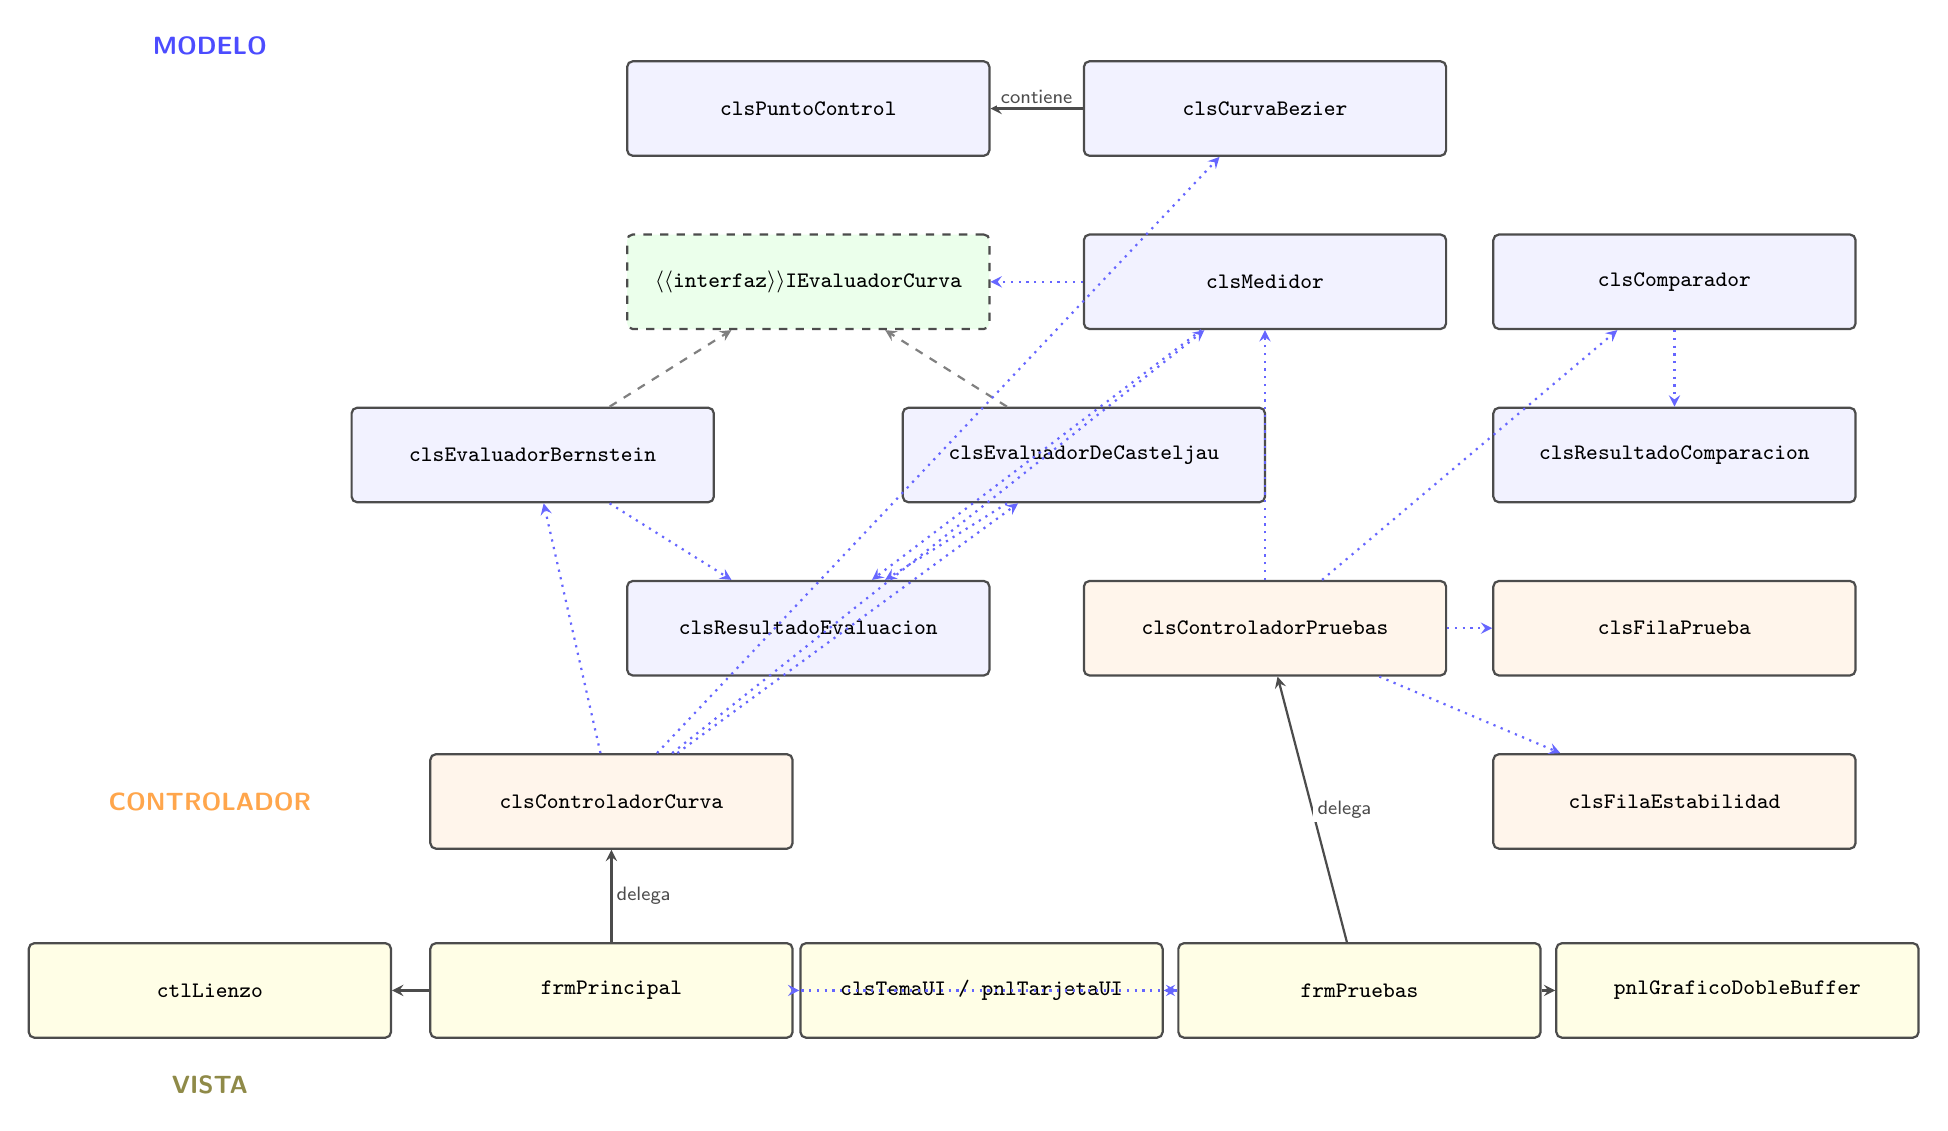
\begin{tikzpicture}[
    clase/.style={rectangle, draw=black!70, fill=blue!5, minimum width=4.6cm, minimum height=1.2cm, text centered, font=\footnotesize\ttfamily, rounded corners=2pt, thick},
    interfaz/.style={rectangle, draw=black!70, fill=green!8, minimum width=4.6cm, minimum height=1.2cm, text centered, font=\footnotesize\ttfamily, rounded corners=2pt, thick, dashed},
    flecha/.style={->, >=stealth, thick, black!70},
    implementa/.style={->, >=stealth, thick, dashed, black!50},
    usa/.style={->, >=stealth, thick, dotted, blue!60},
    etiqueta/.style={font=\scriptsize\sffamily, fill=white, inner sep=1.5pt}
]
% --- CAPA MODELO ---
\node[clase] (puntocontrol) at (0, 0) {clsPuntoControl};
\node[clase] (curvabezier) at (5.8, 0) {clsCurvaBezier};
\node[interfaz] (ievaluador) at (0, -2.2) {$\langle\langle$interfaz$\rangle\rangle$ \\ IEvaluadorCurva};
\node[clase] (bernstein) at (-3.5, -4.4) {clsEvaluadorBernstein};
\node[clase] (casteljau) at (3.5, -4.4) {clsEvaluadorDeCasteljau};
\node[clase] (resultado) at (0, -6.6) {clsResultadoEvaluacion};
\node[clase] (medidor) at (5.8, -2.2) {clsMedidor};
\node[clase] (comparador) at (11, -2.2) {clsComparador};
\node[clase] (rescomp) at (11, -4.4) {clsResultadoComparacion};

% --- CAPA CONTROLADOR ---
\node[clase, fill=orange!8] (ctrlcurva) at (-2.5, -8.8) {clsControladorCurva};
\node[clase, fill=orange!8] (controlador) at (5.8, -6.6) {clsControladorPruebas};
\node[clase, fill=orange!8] (filaprueba) at (11, -6.6) {clsFilaPrueba};
\node[clase, fill=orange!8] (filaestab) at (11, -8.8) {clsFilaEstabilidad};

% --- CAPA VISTA ---
\node[clase, fill=yellow!10] (frmprincipal) at (-2.5, -11.2) {frmPrincipal};
\node[clase, fill=yellow!10] (ctllienzo) at (-7.6, -11.2) {ctlLienzo};
\node[clase, fill=yellow!10] (clstema) at (2.2, -11.2) {clsTemaUI / pnlTarjetaUI};
\node[clase, fill=yellow!10] (frmpruebas) at (7.0, -11.2) {frmPruebas};
\node[clase, fill=yellow!10] (pnldoble) at (11.8, -11.2) {pnlGraficoDobleBuffer};

% --- RELACIONES ---
\draw[flecha] (curvabezier) -- node[etiqueta, above] {contiene} (puntocontrol);
\draw[implementa] (bernstein) -- (ievaluador);
\draw[implementa] (casteljau) -- (ievaluador);
\draw[usa] (bernstein) -- (resultado);
\draw[usa] (casteljau) -- (resultado);
\draw[usa] (medidor) -- (ievaluador);
\draw[usa] (medidor) -- (resultado);
\draw[usa] (comparador) -- (rescomp);
\draw[usa] (ctrlcurva) -- (curvabezier);
\draw[usa] (ctrlcurva) -- (bernstein);
\draw[usa] (ctrlcurva) -- (casteljau);
\draw[usa] (ctrlcurva) -- (medidor);
\draw[usa] (controlador) -- (medidor);
\draw[usa] (controlador) -- (comparador);
\draw[usa] (controlador) -- (filaprueba);
\draw[usa] (controlador) -- (filaestab);
\draw[flecha] (frmprincipal) -- node[etiqueta, right] {delega} (ctrlcurva);
\draw[flecha] (frmprincipal) -- (ctllienzo);
\draw[usa] (frmprincipal) -- (clstema);
\draw[usa] (frmprincipal) -- (frmpruebas);
\draw[flecha] (frmpruebas) -- node[etiqueta, right] {delega} (controlador);
\draw[flecha] (frmpruebas) -- (pnldoble);
\draw[usa] (frmpruebas) -- (clstema);

% --- ETIQUETAS DE CAPA ---
\node[font=\small\bfseries\sffamily, text=blue!70] at (-7.6, 0.8) {MODELO};
\node[font=\small\bfseries\sffamily, text=orange!70] at (-7.6, -8.8) {CONTROLADOR};
\node[font=\small\bfseries\sffamily, text=yellow!50!black] at (-7.6, -12.4) {VISTA};
\end{tikzpicture}
}%
\caption{Diagrama de clases del sistema BezierComparador organizado por capas MVC. Las flechas continuas representan composicion, las discontinuas implementacion de interfaz y las punteadas relaciones de uso.}
\label{fig:impl_diagrama_clases}
\end{figure}

\subsubsection{Responsabilidades de Cada Clase}

En el Cuadro~\ref{tab:impl_clases} se detallan las clases del sistema, su capa MVC correspondiente y sus responsabilidades principales.

\begin{table}[H]
\centering
\caption{Clases del sistema BezierComparador, capa MVC y responsabilidades.}
\label{tab:impl_clases}
\footnotesize
\begin{tabular}{p{3.5cm} l p{8.5cm}}
\toprule
\textbf{Clase / Interfaz} & \textbf{Capa} & \textbf{Responsabilidades} \\
\midrule
\texttt{clsPuntoControl} & Modelo & Encapsula las coordenadas $(x, y)$ de un punto 2D en el plano cartesiano mediante campos \texttt{dblX} y \texttt{dblY} con sus propiedades de acceso. \\
\midrule
\texttt{clsCurvaBezier} & Modelo & Gestiona la lista de puntos de control de una curva de Bezier. Ofrece metodos para agregar, eliminar, modificar y limpiar puntos, asi como para obtener el grado $n = \texttt{Count} - 1$. \\
\midrule
\texttt{IEvaluadorCurva} & Modelo & Interfaz (contrato) que define la firma del metodo \texttt{Evaluar} y la propiedad \texttt{CadNombre}, garantizando intercambiabilidad entre los evaluadores. \\
\midrule
\texttt{clsEvaluadorBernstein} & Modelo & Implementa \texttt{IEvaluadorCurva} evaluando la curva mediante la formula explicita $C(t) = \sum_{i=0}^{n} \binom{n}{i}(1-t)^{n-i}t^i P_i$ con coeficientes binomiales precalculados mediante recurrencia iterativa. \\
\midrule
\texttt{clsEvaluadorDeCasteljau} & Modelo & Implementa \texttt{IEvaluadorCurva} evaluando la curva mediante interpolaciones lineales sucesivas $P_i^{(r)} = (1-t)P_i^{(r-1)} + tP_{i+1}^{(r-1)}$ en arreglos de trabajo. Incluye el metodo \texttt{ObtenerNivelesIntermedios} para visualizar los poligonos intermedios. \\
\midrule
\texttt{clsResultadoEvaluacion} & Modelo & Almacena los puntos calculados de la curva y las metricas de tiempo: promedio, minimo, maximo y desviacion estandar en milisegundos. \\
\midrule
\texttt{clsMedidor} & Modelo & Ejecuta el protocolo de medicion de rendimiento: calentamiento previo (descarte de JIT), $M \ge 10$ repeticiones independientes con \texttt{Stopwatch} y calculo de estadisticas de tiempo. \\
\midrule
\texttt{clsComparador} & Modelo & Calcula la distancia euclidiana punto a punto $d_k$ entre dos curvas evaluadas y reporta el error maximo, el error promedio y el error cuadratico medio (ECM). \\
\midrule
\texttt{clsResultadoComparacion} & Modelo & Estructura de datos que almacena las tres metricas de diferencia numerica entre dos curvas. \\
\midrule
\texttt{clsControladorCurva} & Controlador & Conecta la ventana principal con el Modelo para agregar, mover, buscar y eliminar puntos de control, evaluar ambas curvas en tiempo real, obtener subdivisiones de De Casteljau y ejecutar mediciones con \texttt{Stopwatch}. \\
\midrule
\texttt{clsControladorPruebas} & Controlador & Coordina la ejecucion de los $24$ casos experimentales, genera puntos aleatorios reproducibles con semilla fija, ejecuta la prueba de estabilidad contra referencia \texttt{decimal} de 128 bits y exporta los resultados a CSV. \\
\midrule
\texttt{clsFilaPrueba} & Controlador & Almacena los datos de una fila de resultados: grado, muestras, tiempos de ambos metodos, errores y metodo mas rapido. \\
\midrule
\texttt{clsFilaEstabilidad} & Controlador & Almacena los datos de estabilidad numerica en grados altos: errores de cada metodo frente a la referencia decimal y metodo mas estable. \\
\midrule
\texttt{frmPrincipal} & Vista & Ventana principal interactiva con cabecera de estado, lienzo de trazado (\texttt{ctlLienzo}) y panel lateral de tres tarjetas para puntos de control, configuracion de capas/parametro $t$ y metricas en vivo. \\
\midrule
\texttt{ctlLienzo} & Vista & Control personalizado con doble buffer que dibuja cuadricula CAD, poligono de control, niveles de De Casteljau y ambas curvas empleando exclusivamente \texttt{DrawLine}, \texttt{FillEllipse} y \texttt{DrawString}. \\
\midrule
\texttt{clsTemaUI} / \texttt{pnlTarjetaUI} & Vista & Sistema de diseno centralizado con tokens de color WCAG AA/AAA, tipografia tabular, estados de foco/hover/deshabilitado y paneles tipo tarjeta con doble buffer. \\
\midrule
\texttt{frmPruebas} & Vista & Ventana del laboratorio de pruebas con \texttt{TabControl} en dos pestanas: tabla comparativa de resultados (\texttt{DataGridView}) con resumen de estabilidad, y graficos comparativos exportables a PNG. \\
\midrule
\texttt{pnlGraficoDobleBuffer} & Vista & Panel heredado de \texttt{Panel} con \texttt{DoubleBuffered = true} para evitar parpadeo (\textit{flicker}) durante el redibujado de los graficos. \\
\bottomrule
\end{tabular}
\end{table}

\subsubsection{Convenciones de Nomenclatura: Notacion Hungara en Espanol}
\label{subsubsec:impl_notacion}

Todas las variables, campos, metodos y clases del proyecto siguen la \textbf{notacion hungara adaptada al espanol}, donde cada identificador incluye un prefijo de tres letras que indica su tipo de dato. Esta convencion garantiza la legibilidad inmediata del codigo y la consistencia en todo el equipo de desarrollo. En el Cuadro~\ref{tab:impl_notacion} se documentan los prefijos utilizados.

\begin{table}[H]
\centering
\caption{Prefijos de la notacion hungara en espanol empleados en el proyecto.}
\label{tab:impl_notacion}
\begin{tabular}{llp{7cm}}
\toprule
\textbf{Prefijo} & \textbf{Tipo de Dato} & \textbf{Ejemplo} \\
\midrule
\texttt{ent} & \texttt{int} (entero) & \texttt{entGrado}, \texttt{entMuestras}, \texttt{entRepeticiones} \\
\texttt{dbl} & \texttt{double} (doble precision) & \texttt{dblX}, \texttt{dblTiempoPromedioMs}, \texttt{dblSumaX} \\
\texttt{cad} & \texttt{string} (cadena) & \texttt{cadNombreMetodo}, \texttt{cadMetodoMasRapido} \\
\texttt{bol} & \texttt{bool} (booleano) & \texttt{bolEjecutando} \\
\texttt{obj} & objeto (instancia de clase) & \texttt{objMedidor}, \texttt{objReloj}, \texttt{objResultado} \\
\texttt{lst} & \texttt{List<>} (lista generica) & \texttt{lstPuntosControl}, \texttt{lstResultados} \\
\texttt{arr} & arreglo (\texttt{[]}) & \texttt{arrCoeficientes}, \texttt{arrTiemposMs}, \texttt{arrCurva} \\
\texttt{cls} & clase & \texttt{clsPuntoControl}, \texttt{clsMedidor}, \texttt{clsCurvaBezier} \\
\texttt{frm} & formulario (ventana) & \texttt{frmPrincipal}, \texttt{frmPruebas} \\
\texttt{ctl} & control personalizado & \texttt{ctlLienzo} \\
\texttt{btn} & boton & \texttt{btnMedir}, \texttt{btnEjecutar}, \texttt{btnExportarCsv} \\
\texttt{chk} & casilla de verificacion & \texttt{chkBernstein}, \texttt{chkCasteljau}, \texttt{chkInterpolaciones} \\
\texttt{trk} & control deslizante (\texttt{TrackBar}) & \texttt{trkParametroT} \\
\texttt{lbl} & etiqueta & \texttt{lblEstado}, \texttt{lblGradoActual}, \texttt{lblRepeticiones} \\
\texttt{dgv} & \texttt{DataGridView} & \texttt{dgvResultados} \\
\texttt{pnl} & panel & \texttt{pnlTarjetaUI}, \texttt{pnlGraficoMuestras}, \texttt{pnlSuperior} \\
\texttt{tab} & pestana / \texttt{TabControl} & \texttt{tabContenedor}, \texttt{tabTablaResultados} \\
\texttt{flw} & \texttt{FlowLayoutPanel} & \texttt{flwAcciones}, \texttt{flwFiltros} \\
\texttt{num} & \texttt{NumericUpDown} & \texttt{numMuestras}, \texttt{numRepeticiones} \\
\texttt{cmb} & \texttt{ComboBox} & \texttt{cmbGradoFijo}, \texttt{cmbMuestrasFijas} \\
\texttt{prg} & \texttt{ProgressBar} & \texttt{prgProgreso} \\
\texttt{tip} & \texttt{ToolTip} & \texttt{tipAyuda} \\
\texttt{tbl} & \texttt{TableLayoutPanel} & \texttt{tblInspector}, \texttt{tblGraficos} \\
\texttt{dlg} & dialogo de archivo & \texttt{dlgGuardar}, \texttt{dlgCarpeta} \\
\texttt{col} & color & \texttt{colVerdeGanador} \\
\texttt{dec} & \texttt{decimal} (128 bits) & \texttt{decT}, \texttt{decUnoMenosT} \\
\texttt{pen} & \texttt{Pen} (lapiz GDI+) & \texttt{penBernstein}, \texttt{penCasteljau} \\
\texttt{brs} & \texttt{Brush} (brocha GDI+) & \texttt{brsBernstein}, \texttt{brsTexto} \\
\texttt{fnt} & \texttt{Font} (fuente) & \texttt{fntTitulo}, \texttt{fntEjes} \\
\texttt{bmp} & \texttt{Bitmap} & \texttt{bmpImagen} \\
\bottomrule
\end{tabular}
\end{table}

\subsection{Manual de Usuario}
\label{subsec:impl_manual}

La aplicacion \textit{BezierComparador} inicia en la ventana interactiva \texttt{frmPrincipal}, desde la cual el usuario manipula curvas de Bezier en tiempo real y accede al Laboratorio de Pruebas (\texttt{frmPruebas}). A continuacion se describen las operaciones disponibles.

\subsubsection{Ventana Principal Interactiva (\texttt{frmPrincipal})}
\label{subsubsec:impl_ventana_principal}

La ventana principal se organiza en tres areas principales, como se aprecia en la Figura~\ref{fig:impl_ventana_principal}:

\begin{enumerate}
    \item \textbf{Cabecera superior:} Presenta el titulo de la aplicacion y dos insignias en tiempo real: las coordenadas $(X, Y)$ del cursor sobre el lienzo y el grado actual $n$ junto con la cantidad de puntos de control.
    \item \textbf{Lienzo cartesiano interactivo (\texttt{ctlLienzo}):} Ocupa el area izquierda con cuadricula CAD (lineas menores cada $25\text{ px}$ y mayores cada $100\text{ px}$), leyenda flotante de capas y barra de estado inferior. El usuario puede:
    \begin{itemize}
        \item \textbf{Agregar puntos:} Hacer clic izquierdo en un area libre del lienzo.
        \item \textbf{Mover puntos:} Hacer clic izquierdo y arrastrar cualquier punto de control $P_i$ para deformar la curva en tiempo real (las metricas con \texttt{Stopwatch} se recalculan automaticamente al soltar).
        \item \textbf{Eliminar puntos:} Hacer clic derecho sobre un punto de control existente.
    \end{itemize}
    \item \textbf{Panel lateral de tres tarjetas:} Organizado verticalmente con desplazamiento automatico (\texttt{AutoScroll}) para mantener la responsividad en resoluciones compactas:
    \begin{itemize}
        \item \textit{Puntos de control:} Lista monoespaciada de coordenadas $P_i = (x, y)$, boton \textit{Cargar curva grado 3} y boton \textit{Limpiar lienzo}.
        \item \textit{Configuracion y capas:} Selector numerico de muestras $N$ (\texttt{numMuestras}), casillas de visibilidad por capa (Bernstein, De Casteljau, interpolaciones y poligono de control) y deslizador (\texttt{trkParametroT}) con escala de $0.00$ a $1.00$ para el parametro $t$.
        \item \textit{Metricas de la curva actual:} Tiempos promedio de ambos metodos (10 repeticiones con calentamiento), diferencia maxima, diferencia promedio, ECM, boton \textit{Medir curva actual} y boton verde \textit{Abrir Laboratorio y Graficos Comparativos}.
    \end{itemize}
\end{enumerate}

\begin{figure}[H]
\centering
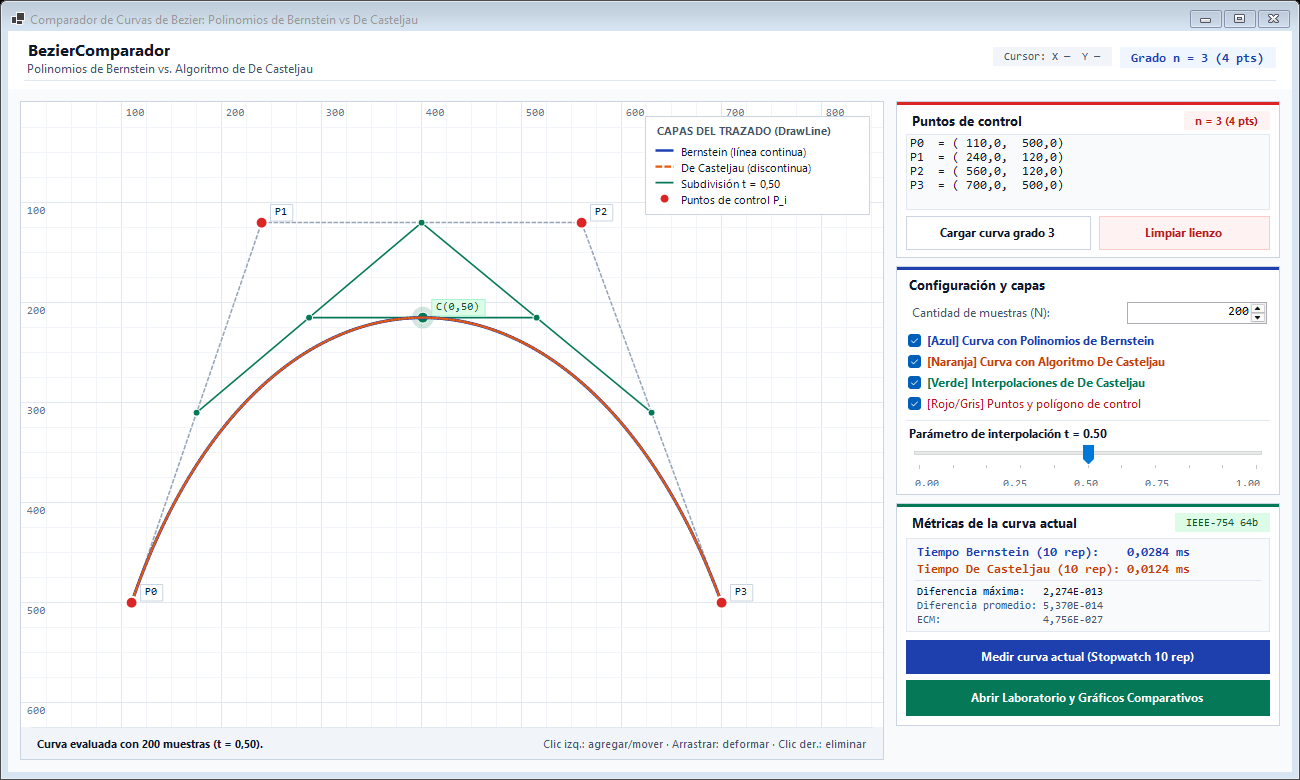
\includegraphics[width=0.95\textwidth]{figuras/impl_ventana_principal.png}
\caption{Ventana principal interactiva de BezierComparador (\texttt{frmPrincipal}) mostrando el lienzo cartesiano, el panel de puntos de control, la configuracion de capas y las metricas en tiempo real.}
\label{fig:impl_ventana_principal}
\end{figure}

\subsubsection{Ejecucion de Pruebas de Rendimiento}
\label{subsubsec:impl_ejecutar}

Al presionar el boton \textit{Ejecutar pruebas}, la aplicacion realiza las siguientes acciones de forma asincrona (sin bloquear la interfaz grafica):

\begin{enumerate}
    \item Deshabilita los controles de entrada para evitar ejecuciones simultaneas.
    \item Itera sobre las $6 \times 4 = 24$ combinaciones de grado y muestras, generando para cada caso un conjunto de puntos de control pseudoaleatorios con semilla fija (\texttt{12345 + n}).
    \item Para cada combinacion, invoca al \texttt{clsMedidor} que ejecuta $M$ repeticiones con calentamiento previo, cronometrando exclusivamente el calculo matematico con \texttt{Stopwatch}.
    \item Calcula las diferencias numericas punto a punto entre ambos metodos con \texttt{clsComparador}.
    \item Actualiza la tabla, ejecuta la prueba de estabilidad en grados $50$ y $100$, y redibuja los graficos.
\end{enumerate}

\subsubsection{Visualizacion de Interpolaciones de De Casteljau}
\label{subsubsec:impl_interpolaciones}

La clase \texttt{clsEvaluadorDeCasteljau} expone el metodo \texttt{ObtenerNivelesIntermedios}, que retorna la lista completa de poligonos intermedios $P_i^{(r)}$ para un valor fijo del parametro $t$. Cuando se activa esta visualizacion, la aplicacion dibuja los segmentos de cada nivel $r$ con colores diferenciados, permitiendo al usuario observar graficamente como la recurrencia de interpolacion lineal converge desde el poligono de control original ($r = 0$) hasta el punto final sobre la curva ($r = n$).

\begin{figure}[H]
\centering
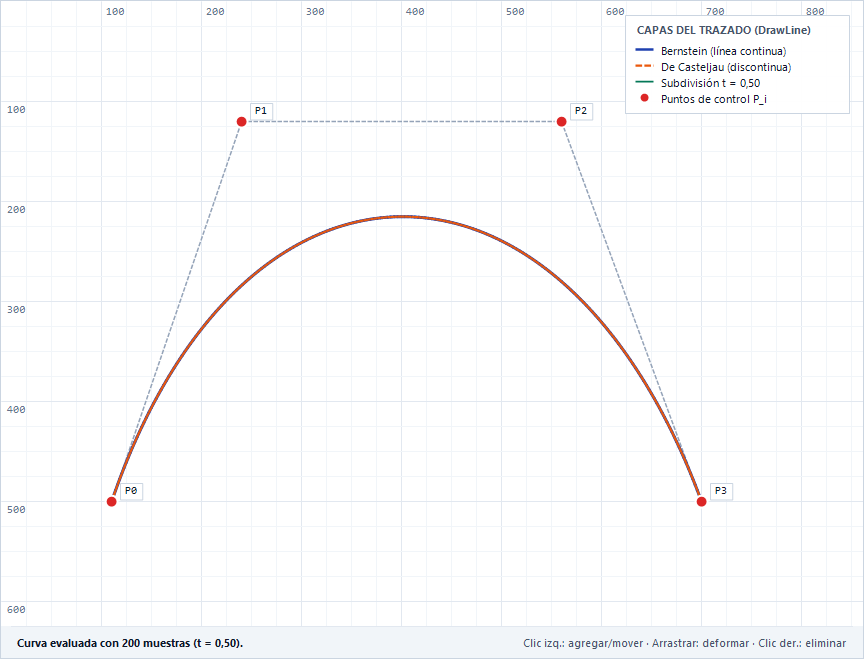
\includegraphics[width=0.88\textwidth]{figuras/impl_curva_grado3.png}
\caption{Curva de Bezier de grado 3 con cuatro puntos de control ($P_0$ a $P_3$), mostrando el poligono de control y las curvas evaluadas por Bernstein (azul continua) y De Casteljau (naranja discontinua) superpuestas.}
\label{fig:impl_curva_grado3}
\end{figure}

\begin{figure}[H]
\centering
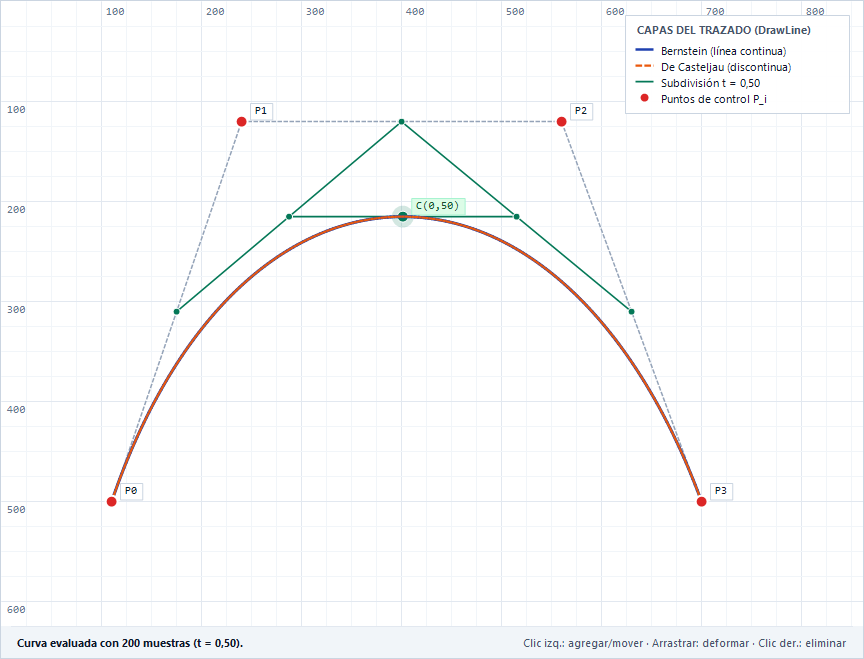
\includegraphics[width=0.88\textwidth]{figuras/impl_interpolaciones.png}
\caption{Interpolaciones de De Casteljau con $t = 0.50$ para una curva de grado 3, mostrando los poligonos intermedios de cada nivel $r$ en verde esmeralda y el punto evaluado $C(0.50)$.}
\label{fig:impl_interpolaciones}
\end{figure}

\subsubsection{Prueba de Estabilidad Numerica}
\label{subsubsec:impl_estabilidad}

El boton \textit{Estabilidad (n=50, 100)} ejecuta la prueba especializada de estabilidad que compara ambos evaluadores en doble precision contra una referencia calculada en aritmetica \texttt{decimal} de 128 bits. Los resultados se presentan en un cuadro de dialogo detallado (\texttt{MessageBox}) que muestra, para cada grado, el error maximo de cada metodo frente a la referencia y el metodo considerado mas estable.

\subsubsection{Exportacion de Resultados}
\label{subsubsec:impl_exportacion}

La aplicacion ofrece dos mecanismos de exportacion orientados a la generacion del informe en \LaTeX:

\begin{itemize}
    \item \textbf{Exportar CSV:} Genera un archivo de valores separados por comas con todas las filas de resultados y las filas de estabilidad, utilizando formato invariante (\texttt{CultureInfo.InvariantCulture}) para garantizar compatibilidad con herramientas de analisis.
    \item \textbf{Guardar PNG:} Renderiza los dos graficos comparativos (\textit{Tiempo vs Muestras} y \textit{Tiempo vs Grado}) en imagenes de $800 \times 480$ pixeles en formato PNG, listas para ser incluidas directamente en el documento \LaTeX\ con \texttt{\textbackslash includegraphics}.
\end{itemize}

\begin{figure}[H]
\centering
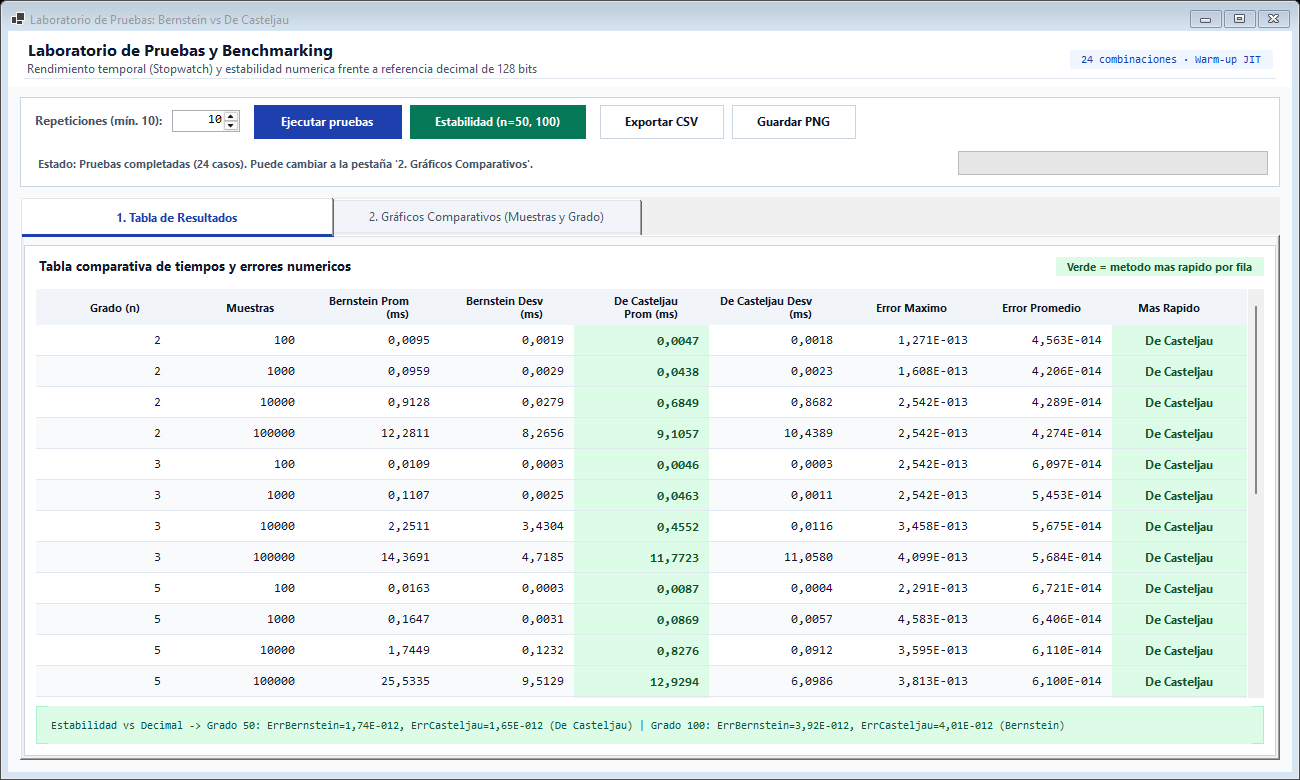
\includegraphics[width=0.95\textwidth]{figuras/impl_ventana_pruebas.png}
\caption{Ventana del Laboratorio de Pruebas (\texttt{frmPruebas}) tras completar la ejecucion de los 24 casos experimentales, mostrando la tabla de resultados con resaltado verde del metodo mas rapido y el resumen de estabilidad numerica.}
\label{fig:impl_ventana_pruebas}
\end{figure}

\subsection{Decisiones de Diseno UI/UX}
\label{subsec:impl_uiux}

El diseno visual y de experiencia de usuario se centralizo en la clase \texttt{clsTemaUI} siguiendo criterios de contraste accesible WCAG AA/AAA, jerarquia visual limpia y consistencia tipografica:

\begin{enumerate}
    \item \textbf{Sistema de tokens de color con significado funcional y contraste WCAG:}
    \begin{itemize}
        \item \textbf{Azul cobalto} (\texttt{\#1E40AF}, contraste $8.59:1$ sobre blanco): Identifica al metodo de polinomios de Bernstein en curvas, botones primarios, pestanas activas y graficos.
        \item \textbf{Naranja quemado} (\texttt{\#C2410C} en texto con contraste $5.18:1$; \texttt{\#EA580C} en trazos): Identifica al algoritmo de De Casteljau.
        \item \textbf{Verde esmeralda} (\texttt{\#047857} en acciones e interpolaciones; fondo \texttt{\#DCFCE7} con texto \texttt{\#14532D} de contraste $8.77:1$): Resalta el metodo mas rapido en la tabla de resultados, el banner de estabilidad numerica y los niveles de subdivision de De Casteljau.
        \item \textbf{Rojo carmesi} (\texttt{\#DC2626}): Representa los puntos de control $P_i$ y la accion de limpieza del lienzo.
        \item \textbf{Superficies Slate neutras:} Fondo general \texttt{\#F8FAFC}, tarjetas \texttt{\#FFFFFF} con bordes \texttt{\#CBD5E1} y tipografia principal \texttt{\#0F172A} (contraste $17.9:1$).
    \end{itemize}

    \item \textbf{Tipografia tecnica y numeros tabulares:} Se combino \texttt{Segoe UI} para encabezados, etiquetas y controles con \texttt{Consolas} monoespaciada para coordenadas, tiempos en milisegundos y errores en notacion cientifica, evitando saltos horizontales al actualizar metricas en tiempo real.

    \item \textbf{Distribucion responsiva con tarjetas y \texttt{TabControl}:} En \texttt{frmPrincipal}, el panel derecho utiliza tarjetas \texttt{pnlTarjetaUI} apiladas dentro de un \texttt{TableLayoutPanel} con \texttt{AutoScroll}. En \texttt{frmPruebas}, se adopto un \texttt{TabControl} con pestanas planas personalizadas (\textit{1. Tabla de Resultados} y \textit{2. Graficos Comparativos}) que aprovecha al maximo el espacio vertical para la tabla y los graficos lado a lado.

    \item \textbf{Accesibilidad, teclado y tooltips:} Todos los controles interactivos definen \texttt{AccessibleName}, \texttt{AccessibleDescription}, orden logico de \texttt{TabIndex}, anillos visibles de foco por teclado (\texttt{\#2563EB}), estados deshabilitados legibles y \texttt{ToolTip} informativos. En el lienzo se muestra retroalimentacion de \textit{hover} y cursor contextual (\texttt{SizeAll} sobre puntos, \texttt{Cross} sobre el plano).

    \item \textbf{Doble buffer (\textit{double buffering}) y renderizado suavizado:} Tanto \texttt{ctlLienzo} como \texttt{pnlGraficoDobleBuffer} y \texttt{pnlTarjetaUI} activan \texttt{DoubleBuffered = true} y \texttt{SmoothingMode.AntiAlias}, eliminando el parpadeo (\textit{flicker}) al arrastrar puntos o redimensionar las ventanas.

    \item \textbf{Graficos y curvas exclusivamente con primitivas basicas y doble codificacion:} Las curvas y los graficos comparativos se dibujan unicamente con \texttt{DrawLine}, \texttt{FillEllipse}, \texttt{FillPolygon} y \texttt{DrawString}. Para no depender unicamente del color, Bernstein utiliza linea continua y marcadores circulares, mientras que De Casteljau utiliza trazo discontinuo en el lienzo y marcadores en forma de rombo en los graficos comparativos.
\end{enumerate}

% RESUMEN: Esta seccion (04_implementacion.tex) documenta las tecnologias (.NET 8/10, C#, WinForms, Stopwatch), la arquitectura MVC actualizada (diagrama TikZ fig:impl_diagrama_clases, tabla tab:impl_clases y notacion hungara tab:impl_notacion incluyendo frmPrincipal, ctlLienzo, clsControladorCurva y clsTemaUI), el manual de usuario completo con las 4 capturas integradas (impl_ventana_principal.png, impl_curva_grado3.png, impl_interpolaciones.png, impl_ventana_pruebas.png) y las decisiones de diseno UI/UX con tokens WCAG AA/AAA.
